% Cherry ds2 — 100k PSNR evaluation
% Build:  pdflatex psnr_evaluation.tex  (run twice)
\documentclass[aspectratio=169,11pt]{beamer}

\usetheme{default}
\usecolortheme{default}
\usepackage[T1]{fontenc}
\usepackage[utf8]{inputenc}
\usepackage{booktabs}
\usepackage{xcolor}
\usepackage{graphicx}

\definecolor{ink}{HTML}{0B0B0B}
\definecolor{ink2}{HTML}{52514E}
\definecolor{zipblue}{HTML}{2A78D6}
\definecolor{fnorange}{HTML}{EB6834}
\definecolor{surface}{HTML}{FCFCFB}

\setbeamercolor{normal text}{fg=ink,bg=surface}
\setbeamercolor{frametitle}{fg=ink,bg=surface}
\setbeamercolor{structure}{fg=zipblue}
\setbeamerfont{frametitle}{size=\large,series=\bfseries}
\setbeamertemplate{navigation symbols}{}
\setbeamertemplate{footline}[frame number]
\setbeamertemplate{itemize items}[circle]
\beamertemplatenavigationsymbolsempty

\newcommand{\zn}{\textcolor{zipblue}{\texttt{fruit\_zipnerf}}}
\newcommand{\fn}{\textcolor{fnorange}{\texttt{fruit\_nerf}}}

\title{ZipNeRF backbone vs.\ FruitNeRF on cherry ds2}
\subtitle{PSNR evaluation of four 100k-step runs}
\author{Nicol\'as Araya}
\date{5 August 2026}

\begin{document}

\begin{frame}[plain]
  \titlepage
\end{frame}

% ------------------------------------------------------------------
\begin{frame}{What was run}
  A $2\times2$ factorial on the same cherry tree capture, all four runs to
  \textbf{100{,}000 steps}, all four finished with
  \texttt{step-000099999.ckpt} on disk.

  \vspace{0.6em}
  \begin{center}
  \begin{tabular}{lll}
    \toprule
    & \textbf{SIFT} & \textbf{ALIKED + LightGlue} \\
    \midrule
    \fn        & \texttt{cherry\_sift\_ds2}  & \texttt{cherry\_aliked\_ds2} \\
    \zn        & \texttt{cherry\_sift\_ds2}  & \texttt{cherry\_aliked\_ds2} \\
    \bottomrule
  \end{tabular}
  \end{center}

  \vspace{0.8em}
  \begin{itemize}
    \item \textbf{Backbone axis:} FruitNeRF's semantic head on Nerfacto vs.\ on a
          ZipNeRF backbone with the \texttt{camp\_zipnerf} recipe
          (\texttt{360\_camp.gin}).
    \item \textbf{SfM axis:} COLMAP with SIFT vs.\ with ALIKED + LightGlue.
    \item Identical frozen dataparser contract, \texttt{downscale\_factor}~$=2$,
          all \textbf{337 frames} registered by both front ends, same eval split.
  \end{itemize}
\end{frame}

% ------------------------------------------------------------------
\begin{frame}{Final PSNR --- full eval set}
  \begin{center}
    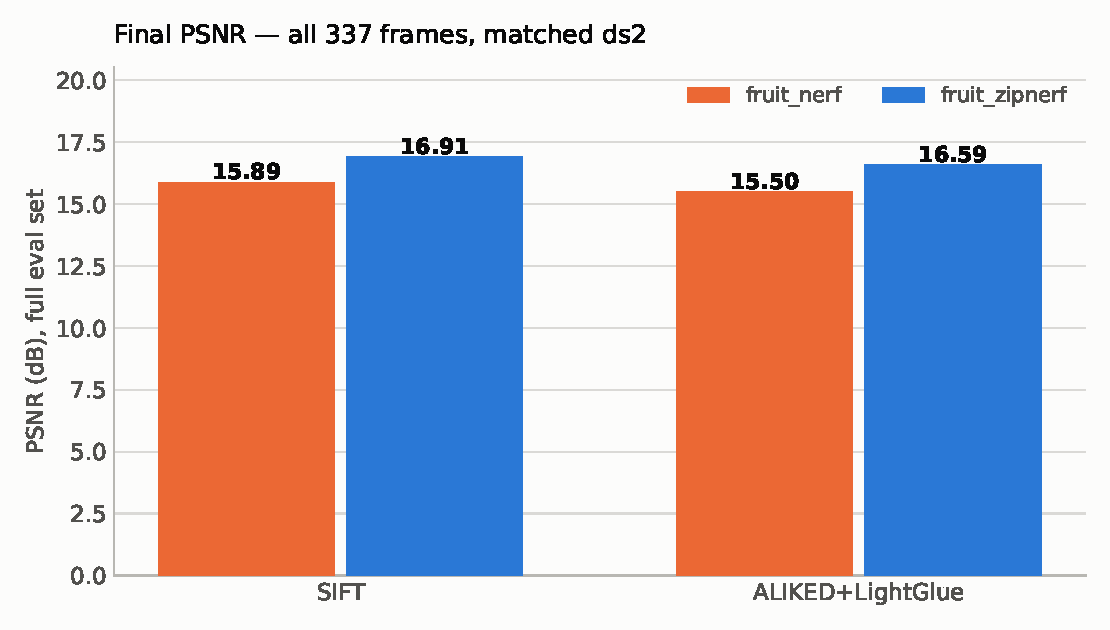
\includegraphics[width=0.82\textwidth]{figs/psnr_final.pdf}
  \end{center}
  \vspace{-0.4em}
  {\small The ZipNeRF backbone is ahead by \textbf{+1.03\,dB} (SIFT) and
   \textbf{+1.09\,dB} (ALIKED) --- consistent in both columns.}
\end{frame}

% ------------------------------------------------------------------
\begin{frame}{All metrics, full eval set (337 frames)}
  \begin{center}
  \small
  \begin{tabular}{llrrrrr}
    \toprule
    \textbf{Front end} & \textbf{Method} & \textbf{PSNR} & \textbf{SSIM} &
    \textbf{LPIPS} & \textbf{sem.\ F1} & \textbf{sem.\ IoU} \\
    \midrule
    SIFT   & \texttt{fruit\_nerf}    & 15.885 & 0.554 & 0.565 & 0.594 & 0.451 \\
    SIFT   & \texttt{fruit\_zipnerf} & \textbf{16.913} & \textbf{0.608} & \textbf{0.520} & 0.592 & 0.461 \\
    \midrule
    ALIKED & \texttt{fruit\_nerf}    & 15.500 & 0.545 & 0.575 & 0.542 & 0.401 \\
    ALIKED & \texttt{fruit\_zipnerf} & 16.585 & 0.591 & 0.558 & 0.539 & 0.420 \\
    \bottomrule
  \end{tabular}
  \end{center}

  \vspace{0.9em}
  \begin{itemize}
    \item PSNR, SSIM and LPIPS all move the same direction: the backbone helps.
    \item Semantic F1 does \textbf{not} move --- $0.594 \to 0.592$ and
          $0.542 \to 0.539$. Both are within noise of each other.
    \item Best overall configuration: \zn{} + SIFT.
  \end{itemize}
\end{frame}

% ------------------------------------------------------------------
\begin{frame}{PSNR over training}
  \begin{center}
    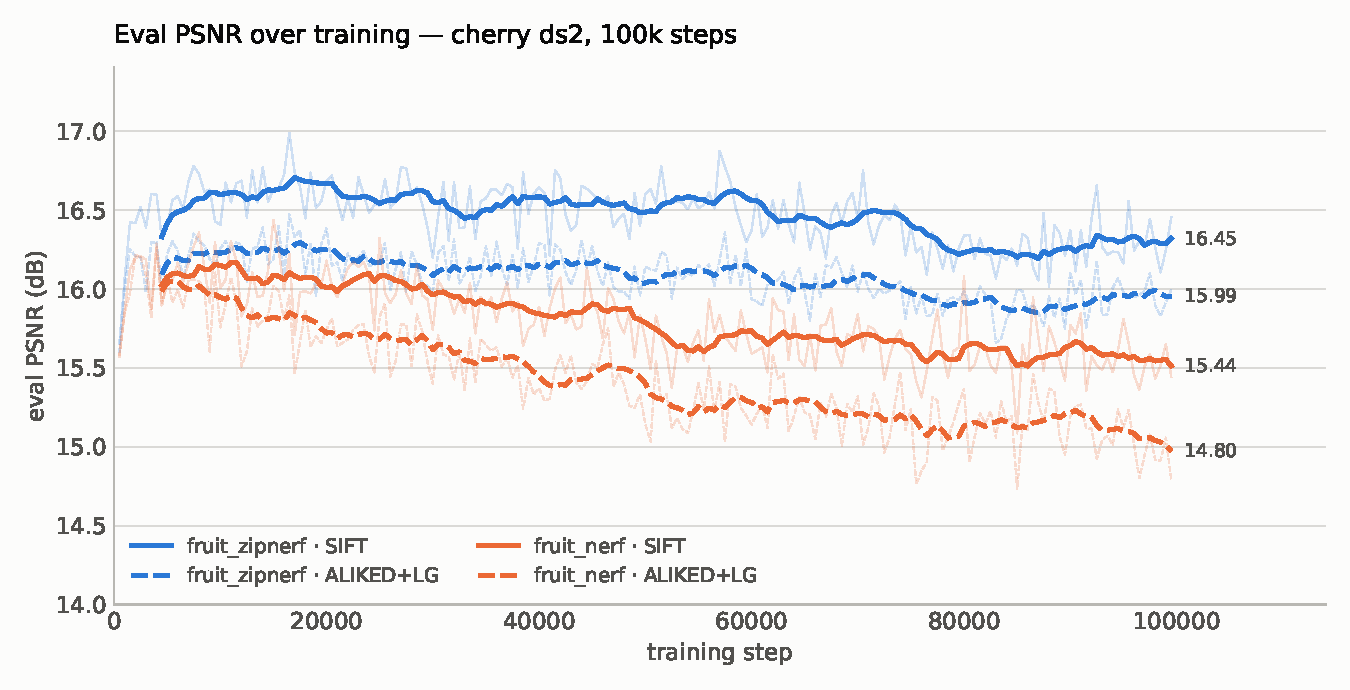
\includegraphics[width=0.86\textwidth]{figs/psnr_curves.pdf}
  \end{center}
  \vspace{-0.6em}
  {\small The ordering is stable from $\sim$5k steps on --- not a late-training
   artifact. But every curve \textbf{peaks near 15--20k, then declines}: 100k is
   past the eval-PSNR optimum for all four.}
\end{frame}

% ------------------------------------------------------------------
\begin{frame}{The SfM axis: better matching, slightly worse NeRF}
  \begin{itemize}
    \item ALIKED + LightGlue produces far more and better keypoint matches than
          SIFT --- established earlier in \texttt{InvNeRF-Seg}.
    \item It nonetheless yields \textbf{lower} PSNR in both backbones:
          $-0.39$\,dB (\texttt{fruit\_nerf}), $-0.33$\,dB
          (\texttt{fruit\_zipnerf}).
    \item Semantic F1 drops more visibly: $0.594 \to 0.542$ and
          $0.592 \to 0.539$.
  \end{itemize}

  \vspace{0.8em}
  \begin{block}{Reading}
    A better SfM front end does not mean a better reconstruction. The effect is
    small and consistent in sign across two independent backbones, which makes
    it more credible than a single run would --- but it is one capture, one
    seed.
  \end{block}
\end{frame}

% ------------------------------------------------------------------
\begin{frame}{Semantic F1 --- where the gain does not reach}
  \begin{center}
    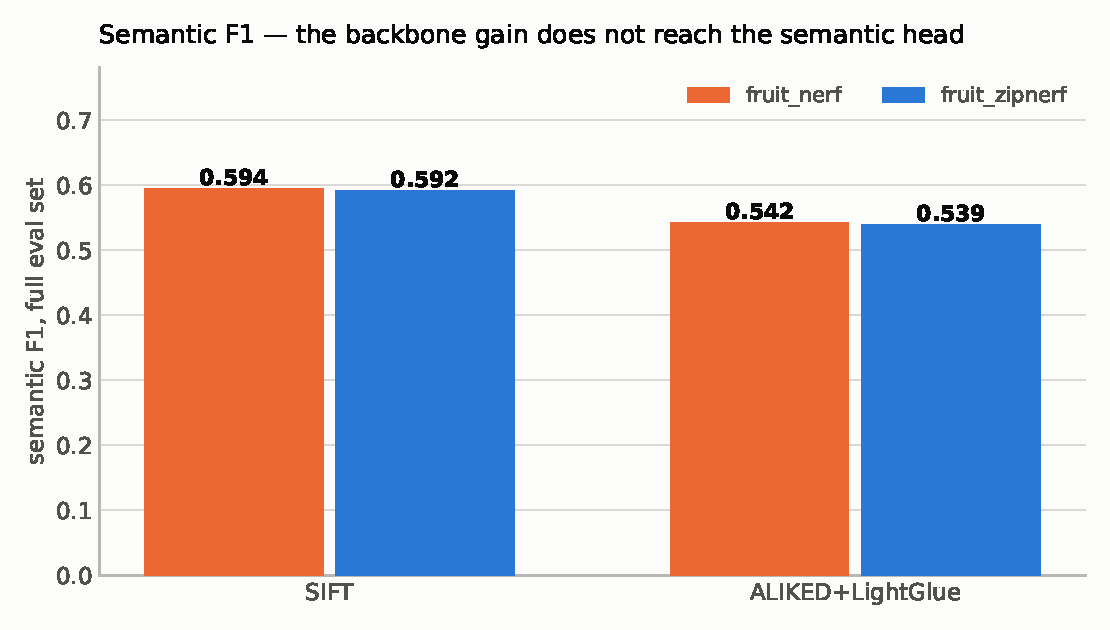
\includegraphics[width=0.80\textwidth]{figs/semantic_f1.pdf}
  \end{center}
  \vspace{-0.4em}
  {\small The backbone changes photometric quality only. The semantic head sees
   nothing: cherry masks cover $\approx 0.53\%$ of each image, and both methods
   use the same unweighted \texttt{BCEWithLogitsLoss}.}
\end{frame}

% ------------------------------------------------------------------
\begin{frame}{Caveats --- read before quoting the $+1$\,dB}
  \begin{enumerate}
    \item \textbf{The LR schedules are not matched.} \fn{} ran 100k steps with
          its upstream default scheduler \texttt{max\_steps}~$=200000$, so its
          LR ended at $\approx 10^{-3}$ instead of its $10^{-4}$ floor --- a
          full decade high. \zn{} used \texttt{max\_steps}~$=100000$ and decayed
          fully. This confound \textbf{favours \zn}.
    \item \textbf{The distortion loss is not matched.} It is computed but never
          added to the loss in \texttt{fruit\_nerf} (inert), while it is a live
          gradient in \texttt{fruit\_zipnerf}. The A/B is therefore not
          backbone-only.
    \item \textbf{One capture, one seed} (\texttt{--machine.seed 42}), no
          repeats --- no error bars on any number here.
    \item PSNR $\approx 16$\,dB is low in absolute terms; $59\%$ of the cherry
          AABB is seen by zero cameras.
  \end{enumerate}
\end{frame}

% ------------------------------------------------------------------
\begin{frame}{Where this leaves the claim}
  \begin{block}{Supported}
    The ZipNeRF backbone reconstructs cherry ds2 better than Nerfacto on every
    photometric metric, in both SfM front ends, by a margin ($\approx 1$\,dB)
    larger than the spread between the front ends.
  \end{block}

  \begin{block}{Not yet supported}
    That the margin is \emph{caused by the backbone}. Two unmatched settings
    (LR schedule, distortion loss) both point the same way as the result.
  \end{block}

  \vspace{0.5em}
  \textbf{Next:}
  \begin{itemize}
    \item Rerun \fn{} with \texttt{scheduler.max-steps 100000} --- one run
          closes the largest confound.
    \item Then the occupancy validation against the InvNeRF-Seg export, with
          deltas checked against the Sim(3) noise floor.
  \end{itemize}
\end{frame}

\end{document}
